\chapter{Implementação}

Neste capítulo descrevemos brevemente o sistema, abordando a organização de seus arquivos componentes e a estratégia de organização do software tendo em vista a criação de uma estrutura de fácil manutenção e expansão.

\section{Visão global}

O jogo é disparado por um pequeno aplicativo cuja única função é iniciar\footnote{Isso foi feito por meio do fork to processo e alteração de suas imagens nos processos pai e filho resultantes.} os componentes Java e C++ do projeto, que passam então a se comunicar via TCP (via \emph{loopback}), empregando a porta de número especificado no arquivo de configuração.

Passada essa etapa de estabelecimento de comunicação, a interação entre C++ e Java se dá pela troca de mensagens, segundo um protocolo simples desenvolvido no trabalho para este projeto em particular. Sua descrição consta no apêndice~\ref{sec:protocolo}. As responsabilidades ficam então assim divididas: a renderização e gerenciamento dos arquivos de diálogos e variáveis do jogo (inventário, membros ativos da gangue, recursos financeiros, etc.) fica a encargo do programa C++, enquanto que toda a tarefa de simulação da arquitetura  BDI e da gerência do blackboard, assim como manutenção do registro dos estados psicológicos, personalidade e conduta dos agentes são de responsabilidade do programa Java (o que inclui o interpretador de AgentSpeak, Jason). Ademais, na arquitetura implementada, o processo Java roda como cliente TCP, e o C++ como servidor.

%Como as coisas funcionam. O que faz o quê (macroscopicamente).

%Uma explicação sucinta da estrutura do programa, como ele inicia
%(forking) e como age em regime (responsabilidades java vs C++, e o
%protocolo).

\section{Compromissos (\emph{trade-offs})}\label{sec:tradeoffs}

Esta seção descreve algumas opções que o grupo fez, sacrificando certos atributos desejáveis em prol de outros no projeto. 

Já foi mencionado que a opção por uma licensa livre para o projeto incorreu tanto em beneífios como em perdas para o projeto. Passou-se a dispor de espaço para hospedagem do projeto, por um lado, embora, por outro, tenha sido necessário abrir mão do uso de engines e bibliotecas proprietárias para o desenvolvimento.

Outro ponto de compromisso foi a decisão por um modelo ``fechado'' de respostas de agentes nos diálogos: a reação dos agentes nesse caso ficou restrita ao conjunto de opções previstas pelo escritor do diálogo. Se por um lado perde-se com a restrição da manifestação do BDI a um conjunto pré-modelado de respostas, por outro ganha-se em condução do diálogo, uma vantagem que não pode ser menosprezada no design do jogo.

Um ponto de destaque foi a decisão de trabalhar com mais de uma linguagem de programação, o fato de trabalharmos com C++, Java e AgentSpeak gerou a necessidade de se desenvolver protocolos de comunicação para integrar os subsistemas, fato este que consumiu bastante tempo e dedicação do grupo.

Por fim, devemos mencionar que, dado o escopo temporal do projeto, optamos por simplificações na sofisticação da renderização. O ganho de tempo dedicado ao projeto veio, nesse caso, às custas de um distanciamento do objeto-alvo de estudo, jogos comerciais, uma vez que o investimento no desenvolvimento de uma apresentação gráfica adequada é uma preocupação constante nesse meio.

\section{Arquitetura}

Conforme descrito anteriormente, a arquitetura do sistema é baseada em dois grandes subsistemas. O subsistema implementado em Java que inclui os códigos interpretados pelo Jason e o subsistema implementado em C++. A figura \ref{arquiteturaGeral} ilustra esta situação.

\begin{figure}
\centering
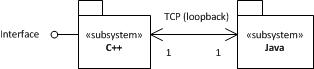
\includegraphics{figuras/arquitetura.jpg}
\caption{Visão geral da arquitetura do sistema}
\label{arquiteturaGeral}
\end{figure}


\subsection{Subsistema: Java}

A figura \ref{arquiteturaJava} apresenta a arquitetura do subsistema implementado em Java. Existem três classes principais, \emph{Manipuladora}, \emph{Comunicadora} e \emph{Level}.
A classe Manipuladora é responsável por consultar e manter atualizados os arquivos de modelos de agentes (explicados em \ref{estruturaPastas}), já a classe Comunicadora é a responsável por receber, enviar e traduzi as mensagens que chegam através da conexão com o subsitema C++. Ambas as classes se comunicam com a classe Level que nada mais é do que a classe de ambiente dos agentes. A classe Level é uma classe utilizada pelo Jason, ela representa o ambiente (enviroment) e é nela que todas as ações dos agentes foram implementadas, no caso deste programa as ações dos agentes são basicamente escolher um tipo de resposta ou atualizar variáveis de controle dos agentes e dos lugares.

\begin{figure}
\centering
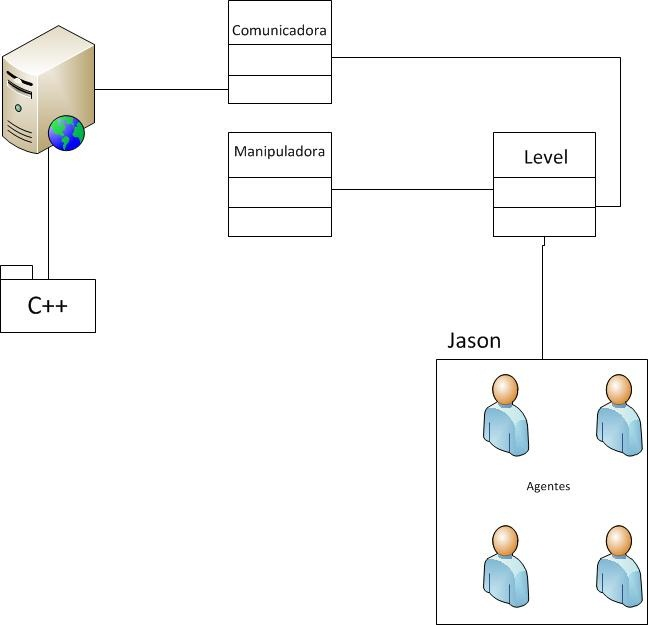
\includegraphics[height=10cm]{figuras/arquitetura-java.jpg}
\caption{Visão geral da arquitetura do subsistema Java}
\label{arquiteturaJava}
\end{figure}

\subsubsection{Arquitetura BDI}
Após pesquisas, o grupo encontrou um \emph{plug-in} do interpretador Jason para rodar com a IDE eclipse, com isto o trabalho ficou mais simples, todo a parte do projeto que utilizava linguagem Java e AgentSpeak foi implementada utilizando a IDE eclipse.
A arquitetura dos agentes não ficou complexa, basicamente todos possuem caracterísicas em comum como a \emph{personalidade} e o \emph{estado psicológico}. No caso de um diálogo estas duas características são necessárias pois é baseado nelas que o agente toma decisões, a atualização destas características ocorre da seguinte forma:
\begin{enumerate} 
\item Classe comunicadora recebe mensagem do tipo estimuloagente ( num agente, num estímulo )
\item Classe Level recebe os parâmetros e insere a crença estímulo(nomeEstimulo) no agente em questão
\item Agente atualiza sua personalidade e seu estado psicológico
\end{enumerate}

Caso o agente receba opções de resposta, ele avalia o(s) estímulo(s) recebido pela fala do jogador e procura a resposta que contenha a reação que lhe interessa, este processo acontece da seguinte forma:

\begin{enumerate} 
\item Classe comunicadora recebe mensagem do tipo estimuloagente ( num agente, num estímulo )
\item Classe Level recebe os parâmetros e insere a crença estímulo(nomeEstimulo) no agente em questão
\item Agente atualiza sua personalidade e seu estado psicológico
\item Classe comunicadora recebe mensagem do tipo ofereceEscolhas( num agente, num reacao1, num reacao2, ... )
\item Classe Level recebe os parâmetros e insere a crença respostas(reacao1,reacao2) no agente em questão
\item O agente procura em sua lógica qual a melhor reação segundo sua personalidade e seu estado psicológico 
\item O agente executa a ação responder(reacao) que envia para o subsitema C++ a escolha do agente
\end{enumerate}

Os casos demonstrados acima se aplicam a qualquer agente com o qual o jogador inicie um diálogo, inclusive os capangas, isto foi feito para manter a arquitetura dos agentes mais genérica.

\subsubsection{Blackboard}

A técnica \emph{blackboard} foi implementada dentro da arquitetura dos agentes ocultos da polícia, esta decisão de projeto visou um melhor desempenho do software.
Basicamente foi criado um agente oculto para cada tipo de informação que pode ser enviada por um agente policial, assim, toda vez que um agente policial executar a ação \emph{avisaPolicia(sujeito,predicado)} é adicionada uma crença em cada agente oculto sobre este aviso, no entanto, apenas um deles sabe o que deve fazer com esta informação, este agente processa a informação e avisa todos os outros agentes a nova informação, esta nova informação pode ser uma ação da polícia que será enviada aos agentes policiais ou pode ser uma nova informação que outro agente oculto sabe processar, assim o processo se torna incremental até que a informação seja completamente processada e resulte em algum tipo de ação da polícia.


\subsection{Subsistema: C++}

A concepção do subsistema C++ foi talvez uma das etapas mais longas do
projeto. Isto pois exite toda uma série de questões inerentes à a organização
do controle da lógica e renderização de jogos, e, como é natural em
sistemas complexos, pequenas decisões da estrutura e organização
refletem grandemente na adequação do sistema à manutenção e
alterações.

Manteve-se em mente durante o pojeto que, dada a novidade do campo de
desenvolvimento de jogos para os integrantes do grupo, dever-se-ia
optar por soluções mais afeitas à modificações. Essa opção é natural,
dado que era grande a probabilidade de que fosse neessário efetuar
modificações para comportar necessidades identificadas ao longo do
desenvolvimento. Ademais, a metodologia de design do jogo escolhida
valia-se de prototipações frequentes, e, nesse sentido, foi importante
que o sistema em si refletisse essa flexibilidade, de modo a atender
às requisições de alteração de comportamento exigidas pela
experimentação com a lógica do jogo. Ressaltamos, entretanto, que essa
flexibilidade não foi total, e desde muito cedo o projeto se fixou em
restrições de apresentação gráfica, numa tentativa de se guardar certo
controle sobre o crescimento da complexidade da renderização do jogo.

Posto de maneira simples, o jogador transita no jogo por estados, como
o \emph{menu principal}\footnote{Menu que permite optar por iniciar um
  novo jogo, carregar um jogo salvo, ou terminar o aplicativo.}, o
\emph{mapa da cidade}\footnote{Mapa por meio do qual o jogador obtém
  acesso à ações como roubar um estabelecimento, fazer compras no
  mercado, etc. (vide o documento de game design, na
  seção~\ref{fluxo-jogo}).}, \emph{diálogos} e \emph{cenas}, 
\emph{gerência de seu inventário de itens}, \emph{compra no mercado} e
\emph{planejamento do roubo}\footnote{Sequência de telas que
  compreende a seleção de participantes do roubo, equipamento a usar,
  e disribuição das recompensas.}. Cada estado é uma abstração de um
conjunto de interações que o jogador pode ter com o jogo.

Foram encapsuladas as primitivas da biblioteca SDL em classes que
\emph{gestoras de recursos}. Esses recursos são
\begin{itemize}
\item imagens (carregadas para serem exibidas na tela,
\item sons,
\item fontes, e
\item eventos.
\end{itemize}

A conexão com o subsistema Java também foi feita encapsulando-se uma
interface SDL, e adaptou-se o sistema interno de captação e
comunicação de eventos do SDL para incorporar as mensagens do
protocolo de comunicação elaborado (vide apêndice~\ref{sec:protocolo}).

Outras abstrações implementadas incluem \emph{design-patterns} como
\emph{decoration}, \emph{strawman}, \emph{singleton}, \emph{factory} e
\emph{interface}. Por exemplo, objetos que queiram ser informados de
eventos do protocolo devem ser \emph{EventListeners} e se inscrever na
lista de ouvintes do \emph{EventManager}, servidor de mensagens do
jogo. Analogamente, objetos que queiram ser desenhados devem ser
\emph{Drawable} e se inscreverem (ou serem inscritos) em alguma
\emph{View} (objetos gerenciadores de exibição de imagens na
tela).

Finalmente, mas não menos importante, o laço principal do jogo
constitui-se da constante medida do tempo decorrido (em milisegundos)
desde a última execução do laço. Este valor é passado para um método
de atualização do gerenciador de estados
(\emph{StateManager}\footnote{Os estados são objetos em uma pilha,
  gerenciada pelo \emph{StateManager}. Ele também é o responsável pela
criação e destruição dos estados.}), que faz o controle da taxa
de atualização da tela.




\section{Protocolo de comunicação}\label{sec:protocolo}

A necessidade de comunicação entre os subsistemas de processamento da inteligência articial implementada e os mecanismos de controle e renderização do jogo surgiram tão logo se foram definidos dois requisitos do projeto, em seu início: o emprego de C++, de modo a refletir um padrão amplamente empregado na indústria de jogos, e a opção pelo uso do interpretador de AgentSpeak, Jason, que possui apenas interfaces para Java.

Definiu-se então um protocolo simples, operando via TCP (\emph{loopback}), o que não incorre em perdas significativas de eficiência na troca de informações. O protocolo, que passou por diversas modificações ao longo da evolução do projeto, baseia-se na troca de mensagens, sequencias de inteiros, que respeitam regras simples:
\begin{enumerate}
\item o primeiro inteiro enviado representa quantos inteiros mais compõe a mensagem;
\item o segundo inteiro identifica o nome da mensagem;
\item os demais inteiros são parâmetros da mensagem.
\end{enumerate}

O nome da mensagem é recuperado pelo receptor da mensagem pela leitura de um arquivo de referência --- é a linha de número igual ao inteiro recebido. Munido dessa cadeia de caracteres, o receptor então pode buscar em um mapa interno a função responsável por tratar a mensagem e seus argumentos. De modo análogo, os argumentos representam, na maior parte das vezes, o número da linha que deve ser lida em algum arquivo do sistema (pré-definido para cada nome de mensagem) contendo algum complemento da informação.

\subsection{Arquivos consultados}

Os arquivos que são lidos pelas rotinas de tratamento das mensagens são
\begin{description}
\item[estímulos] contém estímulos que podem ser enviados a agentes no decorrer de diálogos;
\item[respostas] contém as respostas que agentes podem expressar em diálogos;
\item[capangas] contém nome (e possivelmente outras informações) a respeito de capangas na equipe dos \nomeGrupo;
\item[lugares] contém o nome de lugares passíveis de roubo;
\item[predicados] contém uma lista de avisos que podem ser dados à polícia;
\item[configurações] contém, respectivamente, em suas linhas
\begin{enumerate}
\item o número da porta de comunicação loopback empregado pelos subsistemas em sua comunicação;
\item o número de slots que o jogo possui
\item o maior nível de suspeita possível para capangas (que é também o maior nível de segurança para lugares)
\end{enumerate}
\end{description}

\subsection{Mensagens}

O conjunto de mensagens passou por várias alterações desde sua primeira concepção, o que não somente era esperado, como demonstrou a utilidade da arquitetura de troca de mensagens que havia sido projetada, preparada para acomodar sem grande dificuldade adições e remoções de mensagens. As mensagens são listadas a seguir.

\begin{enumerate}\footnotesize
\item \verb!iniciaDialogo( )! solicita o envio do id de um agente com
  quem o jogador está iniciando um diálogo (o perfil e estado
  psicológico do agente são sorteados pelo subsistema Java);
\item \verb!retornaIdAgente()! retorna um id solicitado por \verb!iniciaDialogo()!;
%
\item \verb!estimuloagente ( # agente, # estímulo )! estimula o agente
  referido;
%\item \verb!atualizaBeliefs(# agente, # estimulo)! 
%
\item \verb!ofereceEscolhas( # agente, # reacao1, # reacao2, … )!
 lista uma série de reações que o agente pode expressar;
\item \verb!returnEscolha(# agente, #escolha)! retorna a escolha
  escolhida pelo agente como a que mais se aproxima de expressar seu
  estado psicológico atual;
%
%
\item \verb!fimDialogo( #agente )! avisa o término do diálogo;
\item \verb!acaoDaPolicia( #acao, #alvo )! solicita ao jogo que tome
  alguma ação em nome da polícia; ações previstas incluem
  \begin{itemize} 
  \item  aumentar nivel suspeita de capanga (alvo);
  \item  diminuir nivel suspeita de capanga (alvo);
  \item  prender  capanga (alvo);
  \item  aumentar nivel segurança de lugar (alvo);
  \item  diminuir nivel segurança de lugar (alvo);
  \end{itemize}
%
\item \verb!avisaPolicia( #sujeito, #predicado )! informa a polícia de
  algo:
  \begin{itemize}
  \item alguém fez compra suspeita;
    \item tentativa de roubo (sucesso);
      \item tentativa de roubo (sucesso);
  \end{itemize}
\item \verb!avisaPolicia( #sujeito, #predicado, #alvo )! informa a
  polícia de algo sobre alguém;
  \begin{itemize}
  \item alguém agiu de modo suspeito em um dado lugar;
  \end{itemize}
%[10 escreveBlackBoard(#sujeito, #predicado)] => 8
%
\item \verb!loadGame(! \#slot \verb!)! solicita carga de jogo;
\item \verb!newGame(! \#slot \verb!)! solicita novo jogo;
\item \verb!saveGame(! \#slot \verb!)! sollicita salvamento de jogo
\item \verb!quitGame()! informa fim de jogo.
\end{enumerate}

A concepção do protocolo de comunicação envolveu alguns cuidados especiais, e precauções foram tomadas no sentido de preservar a flexibilidade do protocolo --- isto é, facilitar a adição de novas mensagens no decorrer do projeto --- e garantir certo desacoplamento entre o trabalho de modelagem de agentes e projeto do blackboard, de um lado, e a lógica do jogo, de outro. Buscou-se organizar a comunicação entre Java e C++ de modo tal que o projeto pudesse ser levado a cabo sem a necessidade de programadores de um e outro sistema precisassem saber do funcionamento do outro. Essa flexibilidade permite que as responsabilidades dos sistemas sejam alteradas durante a evolução do projeto, o que é importante para permitir a exploração de possibilidades de organização do jogo como um todo. Para isso, é necessário que os protótipos construídos não enfrentem as restrições de uma arquitetura rígida.

\section{Estrutura de pastas}\label{estruturaPastas}

O projeto foi desenvolvido com vistas a se prestar à experimentação no
design. Assim, algumas ferramentas para a escrita de \emph{scripts} de
diálogos ou pequenas cenas foram desenvolvidas.

Descrevemos a seguir a organização dos arquivos do projeto. É
importante que essa estrutura seja clara e intuitiva, já que é nossa
intenção que alguns desses arquivos (que configuram o comportamento
do jogo) sejam alterados primariamente por designers do jogo. Assim, é
preciso que haja critério na complexidade que se expõe a esses
``usuários''. A figura~\ref{fig:estrut-arquiv} exibe a distribuição de arquivos nas pastas do projeto.  

\begin{figure}
\centering
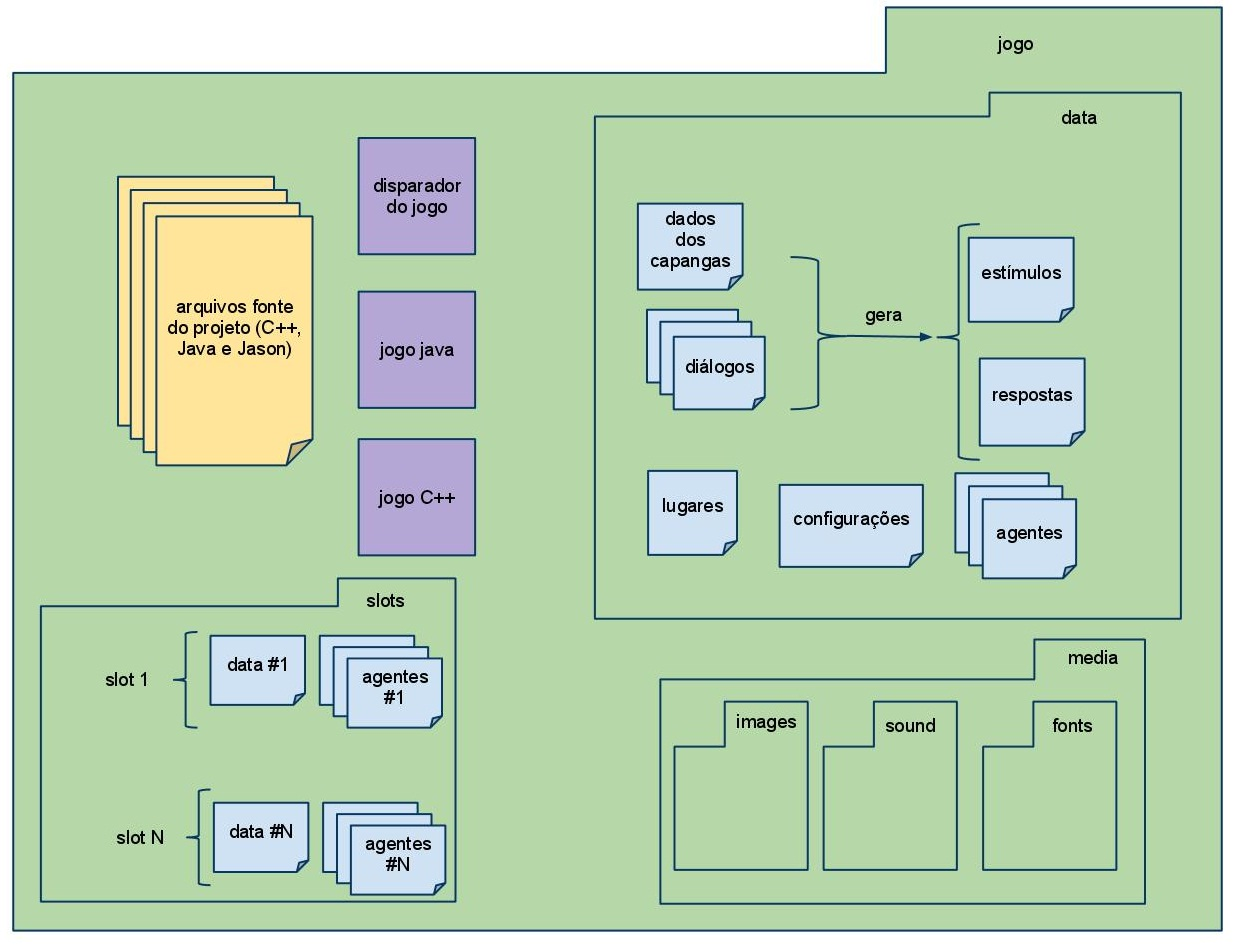
\includegraphics[width=\textwidth]{figuras/estrutura-arquivos.jpg}
\caption{Organização de arquivos do projeto}
\label{fig:estrut-arquiv}
\end{figure}


\section{Arquivos auxiliares}

Uma série de arquivos de texto auxiliares são usados pelo jogo. São em sua maioria estáticos, sendo que alguns são lidos por ambos os programas. Ressalta-se que os conjuntos de arquivos gerados por Java e C++ não têm intersecção, o que elimina a necessidade de gerência de situações de escrita concorrente. Eles especificam:
\begin{itemize}
\item diálogos,
\item modelos de agentes,
\item informações de instâncias de agentes,
\item tipos de reações,
\item tipos de estímulos a agentes,
\item lugares passíveis de assalto,
\item dados de capangas,
\item ações da polícia.
\end{itemize}

Explicamos a seguir a função de cada um dos tipos de arquivo.

Os \emph{modelos de agentes} são arquivos de texto para controle das informações de cada agente. Possuem as seguintes informações sobre os agentes:
\begin{itemize}
\item tipo do agente: inteiro que define o tipo do agente (0-capanga,1-civil,2-policial,3-oculto).
\item id do agente: inteiro único, entre 10 e 99 que representa o agente.
\item nome do agente: String com o nome do agente.
\item personalidade: String que define a personalidade atual do agente.
\item estado psicologico: String que define o estado psicológico atual do agente.
\end{itemize}
Os itens listados acima são comuns a todos os tipos de agentes.
Além dos itens listados acima, os arquivos de agentes policiais possuem uma informação extra sobre a variável \emph{conduta} associada a cada policial, que é uma String que pode assumir dois valores (ganancioso ou íntegro), e os arquivos de agentes capangas possui a variável \emph{nível de suspeita} que é um inteiro (o valor máximo desta variável é definido no arquivo de configuração), ela serve para a polícia monitorar os capangas e decidir se deve ou não prendê-lo.
Vale citar que existe um arquivo por agente e que o nome do arquivo é sempre formado pela seguinte regra: \verb!a! + \verb!tipo-do-agente! + \verb!id-do-agente.txt!

Os \emph{tipos de estímulos, tipos de reações, lugares passíveis de assalto, dados de capangas,} e \emph{ações da polícia} são arquivos de interface, lidos por ambos os programas na decodificação de mensagens trocadas. Optou-se por essa solução para que a comunicação se desse pelo envio de inteiros, indicando qual a linha do arquivo de interface
em que a mensagem está contida. Com isso o processo de alteração do protocolo em seus estágios iniciais de desenvolvimento foi simplificado, uma vez que sua própria especificação atua como um tipo de documentação. Além disso, a mudança das mensagens do protocolo passou a ser feita pela mudança de algumas linhas em um arquivo de configuração e em um mapa de strings a funções, o que facilitou a experimentação. Claramente, essa abordagem só é
possível porque as mensagens são conhecidas \emph{a priori}.

Para comunicar o estímulo que uma determinada fala no diálogo provoca
no agente, a lógica do jogo envia ao sistema BDI um inteiro indicando
a linha em que está escrita a string que define o estado. Na prática,
a lógica do jogo faz uma chamada para enviar o inteiro correspondente
ao estímulo que se deseja comunicar, e uma busca é feita no arquivo
que contém os estímulos possíveis para encontrar o conteúdo da linha
correspondente. Essa string é, por fim, enviada ao sistema BDI, que
fará a sua própria busca para identificar qual o estímulo recebido.

Vale notar que os arquivos contendo os estímulos e reações são gerados por um programa que os extrai dos diálogos escritos para o jogo.

Os \emph{diálogos} são scripts que codificam possíveis dizeres que
\npc{}s ou o jogador podem efetuar em um diálogo. Carregam informação sobre
o sentimento que expressam ou a impressão que causam. 
O grupo desenvolveu uma gramática de scripts específica para os diálogos.

\subsection{Cenas e \emph{scripts} de diálogos}
Scripts, em geral, constituem parte da interface entre os times de
desenvolvimento, arte e dessign de games. Muito se discute, nesse
meio, quanta complexidade é interessante que os programadores deixem
acessível por meio do script que criaram. Complexidade em demasia via
de regra vem acompanhada de estruturas elaboradas de programação, com
duas consequências negativas que vale a pena citar
\begin{itemize}
\item aumento no tempo gasto implementando o interpretador de scripts,
\item risco de ocorrer delegação de tarefas da equipe de
  desenvolvimento para as demais.
\end{itemize}

É certo que, usados com parcimônia, os scripts são uma ferramenta
fundamental na dinamização do processo de testes e experimentação
durante a confecção do jogo, e o resultado, é o que alguns chamam
de~\emph{design orientado a dados}, ou~(\emph{data-driven design}).

Nesta seção abordamos duas linguagens de scripts feitas, para controle
de ``filmes'' exibidos durante o jogo, e para composição de diálogos.

\subsubsection{Script de cenas}

Adoou-se uma simplificação no tipo de cena que seria o jogo
comportaria. As cenas são uma sequência de imagens e texto,
acompanhadsd de música --- algo similar a apresentações de slides. Eis
um pequeno exemplo de script.

{\centering
\footnotesize
\begin{verbatim}
<music=musica-de-fundo.mp3>
<background=imagem-de-fundo-1.jpg>
<>Uma ideia brilhante
<wait=1000>
<>Uma ideia brilhante.
<wait=1000>
<>Uma ideia brilhante..
<wait=1000>
<>Uma ideia brilhante...
<wait=2000>
<fadeOut=500>
<background=imagem-de-fundo-2.jpg>
<fadeIn=100>
<>Um projeto
<wait=1000>
<>Um projeto re
<wait=600>
<>Um projeto revo
<wait=600>
<>Um projeto revolu
<wait=300>
<>Um projeto revolucio
<wait=600>
<>Um projeto revolucioná
<wait=600>
<>Um projeto revolucionário!
<wait=2000>
<fadeOut=2000>
<background-color=black>
<>Porém...
<fadeIn=500>
<wait=4500>
<fadeOut>
\end{verbatim}
}

O exemplo acima foi construído para exibir as principais
características do script feito. Primeiro, inicia uma música de fundo,
acompanhada de uma imagem ao fundo. A seguir, uma sequência de frases
é exibida, de modo que fique a impressão de que letras são adicionadas
pouco a pouco. A seguir a tela escurece, prepara-se uma outra imagem
de fundo para substituir a anterior, e o mesmo efeito de substituição
do texto por um texto parecido é empregado para enfatizar a palavra
``revolucionário'', que aparece sílaba por sílaba, a intervalos de
$600$ milisegundos. A tela então escurece novamente, e prepara-se a
exibição de uma tela preta com os dizeres ``Porém\ldots'', que então
aparecem em uma transição de $500$ms. Por fim, após $4,5$ segundos a
tela escurece novamente e a cena termina.

\subsubsection{Script de diálogos}
Descrevemos a seguir a gramática da linguagem de especificação de diálogos.
Os diálogos são criados através de uma linguagem de marcação muito parecida com a linguagem \emph{xml}. Todas as instruções são descritas no começo da linha na seguinte forma: \emph{$<$instrucao1 instrucao2 … instrucaoN$>$ texto}. Vale citar que uma fala pode não ser precedida por nenhuma instrução, representada por \emph{$<>$}, nesse caso a fala, seja ela do jogador ou do \npc{} é simplesmente apresentada. A marcação de fim do diálogo é feita através da sequência $<$/$>$.
Cada diálogo é completamente escrito em um arquivo, sendo assim, quando o jogador inicia um diálogo, somente um arquivo é utilizado e neste arquivo, a primeira fala será sempre a do jogador.

A grande funcionalidade da linguagem criada é que ela oferece, de forma simples, opções de falas tanto para o jogador quanto para o \npc{}. Toda vez que for encontrada a sequência \emph{$<$opts$>$} significa que foi aberta uma parte do diálogo, e é possível ao jogador ou ao \npc{} escolher mais de uma fala. As opções são listadas ao lado da sequência \emph{$<$op$>$}, e ao final da lista de opções deve existir a sequência de fechamento \emph{$<$/opts$>$}.

Outro aspecto interessante da linguagem desenvolvida é a existência de desvios no rumo do diálogo, o desenvolvedor pode dividir o arquivo em blocos de um mesmo diálogo separados por \emph{labels}, como por exemplo, \emph{$<$label sucesso$>$ . . . $<$/$>$} e desviar o diálogo para este bloco através de uma instrução do tipo \emph{$<$goto=sucesso$>$} onde \emph{``sucesso’’} é um label associado a um bloco do diálogo que só será acessado se o jogador ou o \npc{} selecionar uma fala que contenha a instrução descrita acima.

A principal característica da linguagem desenvolvida é que com ela é possível passar ao \npc{} o estímulo que a fala irá produzir, por exemplo \emph{$<$op elogio$>$ voce é linda!}, com isso o \npc pode considerar possíveis opções de resposta, estas por sua vez estão associadas à reações que são descritas da mesma maneira, por exemplo \emph{$<$op agradecer$>$ obrigado!}. 

Além disso, dois detalhes interessantes foram adicionados, um comando que associa uma cor a uma fala do \npc{} e um comando de liga/desliga que pode ser utilizado por exemplo para habilitar/desabilitar itens para o jogador. O fato da cor associada a fala do \npc{} mudar é interessante pois a cor será um tipo de \emph{feedback} para o jogador ter uma noção de como o \npc{} está se sentindo. O comando tem a seguinte sintaxe: \emph{$<$color=cor$>$}, onde a variável cor pode assumir três valores, green (\npc{} está gostando), yellow (\npc{} está apreensivo) ou red (\npc{} não está gostando), além disso, caso o \npc{} esteja indiferente, nenhuma cor é associada à caixa de texto de sua fala. 

O comando para ligar/desligar é da forma \emph{$<$SWITCHON=x$>$} para ativar qualquer coisa que seja representada pela variável \emph{x} ou {$<$SWITCHOFF=x$>$} para desativar.

O último comando que deve ser apresentado é o comando \emph{$<$only=DadoCapanga$>$texto} onde a variável \emph{DadoCapanga} representa algum atributo descrito no arquivo de modelo do capanga em questão. Desta forma, a fala em questão só estará disponível para o jogador se a condição do comando for verdadeira.

A seguir apresentamos um exemplo de um texto de diálogo entre o jogador e um \npc{}. Neste caso, se o jogador tiver sucesso ele destrava um item, ou até mesmo ganha este item, senão não terá acesso ao item e pode até mesmo ter o nível de suspeita de seu capanga incrementado.
%Para facilitar o entendimento, as linhas azuis representam as falas disponíveis ao jogador e as linhas pretas as falas disponíveis ao \npc{}.

{\footnotesize
\begin{verbatim}
<! Diálogo entre homens para liberar sonífero / se tornar suspeito >
<opts>
  <op fala-amigavel>Bom dia, senhor.
  <opts>
    <op> Bom dia.
    <op> Olá.
    <op goto=rabugento rabugento color=yello> Bom dia pra quem?!
    <op goto=rabugento rabugento color=yellow> Hmpf, o que o senhor quer?
    <op apressado> Desculpe, estou sem tempo para conversar.
    </>
  </opts>
  <op insulto>E aí véio?
  <goto=retratacao color=red effect=shaking>Quem é velho?
  <op only=EngProd  fala-amigavel elogio>Está um belo dia hoje não?
  Tão belo quanto o senhor!
</opts>

<opts>
  <op inquisitivo>Você trabalha aqui?
  <opts>
    <op goto=sonifero> Não, trabalho na farmácia!
		
		<op goto=sonifero>Não, sou farmacêutico!
		<op apreensivo color=yellow> Por que você quer saber?
	</opts>
<op>Você tem horas?
<>Erm, não...
</>
</opts>
</>
<label retratacao>
<opts>
	<op insulto>Não ouviu? Eu disse E AÍ SURDO!?
	<opts>
<op color=red> Que absurdo!
	<op irritado color=red>Vá se danar!
</opts>
	</>
	<op>Perdão, pensei que fosse um amigo meu. Mas nossa, vocês
são muito parecidos!
	<opts>
		<op only=EngProd>Curioso, você não é o primeiro a me
dizer isso...
		<>Sério? Seria incrível então se o senhor também
trabalhasse com...
		<>Farmácia?
		<>Caramba, isso é que é coincidência! Por falar nisso,
eu estava indo para uma agora...
		<>Doente, por algum acaso?
		<>Bom, não exatamente. Insônia. Faz duas semanas que
eu não consigo dormir direito.
		<switchOn=dormeflex goto=terminabem color=green>Já
sofri disso, é um incômodo. Aceita uma sugestão? Use o  "dormeflex",
vende na farmácia aqui perto.
		<op>Pois é... bom, tchau!
</>
	</opts>

<label sonifero>
<opts>
	<op only=EngProd elogio> Sério? Você caiu do céu!! Você não
teria um remédio para me ajudar a dormir teria?? Tenho sofrido muito
com essa insonia!
	<opts>
	<op goto=enecrraBem feliz SWITCHON=dormeflex color=green>
Claro! 			Também sofro com este problema! Na verdade,
tenho uma pílula aqui no 			bolso, pode levar!!
<op goto=encerraBem  lisonjeado SWITCHON=dormeflex color=green>
Caí do céu?? Que isso, foi pura coincidência! Mas  eu tenho o  remédio
que você precisa, te vendo por um precinho amigo! quer comprar?
<op goto=encerraBem SWITCHON=dormeflex color=green>
Certamente! Passe no mercado e compre um "dormeflex"!
</opts>
	<op suspeito> O senhor vende remédios para fazer alguem
dormir?
	<opts>
		<op apreensivo color=yellow> Claro que sim! Mas por
que o senhor 				desejaria fazer alguém dormir?
<op goto=encerraBem SWITCHON=dormeflex color=green> Vendo sim!
Passe no mercado e compre uma pílula de "dormeflex"! Derruba
elefantes!
</opts>
	<opts>
	<op insulto> Não lhe interessa!
	<op insulto> Pra "alguém" dormir!
	<op fala-amigavel> É para minha esposa! Ela sofre de insônia!
	<op only=EngProd inquestionavel> Vou ser sincero! É para minha
esposa, amanhã tem final do futebol! Preciso que ela durma senão não
posso ver o jogo em paz!!
</opts>
	<opts>
	<op goto=encerraBem SWITCHON=dormeflex compreensivo
color=green> Muito justo o seu motivo! Aqui está, coloque na
bebida dela ou na comida e ela vai dormir a noite toda!
	<op goto=encerraMau color=red> Que absurdo! O senhor quer
drogar sua própria esposa?! Não posso e nem quero participar
disto!
</opts>
	
	<op insulto> Ou, descola uns remédios para dormir pra mim??
		<opts>
			<op goto=encerraMau zangado color=red>  De
jeito nenhum!
			<op goto=encerraMau rabugento color=red> Não
sou traficante 					"mano"!
			<op goto=encerraBem SWITCHON=dormeflex
color=green> 					Compra lá no mercado
uns "dormeflex".
</opts>
</opts>
</>

<label encerraBem>
<! fala do jogador>
	<opts>
		<op fala-amigavel> Muito obrigado!
		<op elogio> O senhor salvou minha vida!! Obrigado!
</opts>
<color=green> Que isso!? É um prazer ajudar! Me procure sempre que
precisar! Até mais!
</>

<label encerraMau>
	<opts>
		<op insulto> Muito obrigado! Por não me ajudar em nada!
		<op fala-amigavel> Desculpe incomodá-lo!
</opts>
<opts>
	<op educado> Sinto muito! Não posso ajudá-lo!
	<op zangado color=red> Veremos o que a polícia acha disso?
	<op apreensivo color=red> Não quero nada com isso!!
	<op> Adeus senhor!
</opts>
</>
\end{verbatim}
}


